\documentclass[12pt,a4paper]{extarticle}
\usepackage{../templates/preamble}

\renewcommand{\typeof}{Пояснительная записка к курсовой работе\par}
\renewcommand{\papertheme}{Использование списков для создания справочника учёта\par исполнителей и выполненных работ\par и навигации по нему.}

\begin{document}
\input{../templates/titlepage.tex}
\setcounter{page}{2}


\begin{center}
    ЗАДАНИЕ НА КУРСОВУЮ РАБОТУ
\end{center}

Студент Даричев Е.М.\par Группа 4352

\begin{center}
    Тема работы:
\end{center}

Использование списков для создания справочника учёта исполнителей
и выполненных работ и навигации по нему.

\begin{center}
    Исходные данные:
\end{center}

Проводится учет выполнения работ разного вида несколькими
исполнителями. Требуется хранить информацию об исполнителях (ФИО, адрес,
табельный номер), о работах (наименование, исполнители, норма на
исполнителя/-ей, тариф) и о выполненных работах (исполнители, наименование,
объем, дата завершения). Надо обеспечить возможность получения:
\begin{itemize}
    \item общего списка работ и их исполнителей,
    \item списка выполненных работ на конкретную дату/период (группировка по
    исполнителям и/или видам работ),
    \item работ, выполненных одним исполнителем,
    \item есть ли работы, выполненные одной и той же группой исполнителей.
    Для выполненных работ должна подсчитываться стоимость работ.
\end{itemize}
\begin{center}
    Содержание пояснительной записки:
\end{center}

«Оглавление», «Введение», «Основная часть», «Заключение».
\begin{center}
    Предполагаемый объем пояснительной записки: не менее 30 страниц.
\end{center}

Дата выдачи задания: 17.02.2025
Дата сдачи:
Дата защиты:

\vspace{\fill}
\thispagestyle{empty}
\begin{table}[h!]
    \centering
    \begin{tabularx}{\textwidth}{p{60mm}X>{\centering\arraybackslash}p{45mm}}
        Студент гр. 4352 & \_\_\_\_\_\_\_\_\_\_\_\_\_\_\_\_\_\_\_\_ & {Даричев Е. М.} \\ [5.4mm]  % Line height
        Преподаватель    & \_\_\_\_\_\_\_\_\_\_\_\_\_\_\_\_\_\_\_\_ & {\teacher} \\ [5.4mm]
    \end{tabularx}
\end{table}

\newpage

\begin{center}
    АННОТАЦИЯ
\end{center}

В курсовой работе представлена программа, организовавшая справочник по работам и их
исполнителям. Данные хранятся в рекурсивных списках: работа включает в себя исполнителей,
а исполнитель включают в себя работы. Обеспечена выдача данных о задачах по особым запросам:
в промежутке дат, по исполнителям и группам исполнителей. Все названия и имена хранятся в виде
однонаправленных списков, состоящих из блоков статичной длины. Сведения читаются из файлов.
Управлять выводом можно с помощью консольного меню. Действия программы по считыванию хранятся в
протоколе, а результаты запросов записываются в файл выхода.

\begin{center}
    SUMMARY
\end{center}

The term paper presents a program that implements a directory of tasks and their executors.
The data is stored in recursive lists: a task includes executors, and a executor includes tasks.
The program provides information about tasks based on specific queries: within a date range, by executors
and groups of executors. All names and titles are stored as singly linked lists consisting of blocks
of fixed length. Data is read from files. Output is controlled via a console menu. Actions performed
by the program are logged in a protocol file, and query results are written to an output file.

\newpage
\tableofcontents
\newpage

\section*{ВВЕДЕНИЕ}
\section{Исходная формулировка задания}
Проводится учет выполнения работ разного вида несколькими
исполнителями. Требуется хранить информацию об исполнителях (ФИО, адрес,
табельный номер), о работах (наименование, исполнители, норма на
исполнителя/-ей, тариф) и о выполненных работах (исполнители, наименование,
объем, дата завершения). Надо обеспечить возможность получения:
\begin{itemize}
    \item общего списка работ и их исполнителей,
    \item списка выполненных работ на конкретную дату/период (группировка по
    исполнителям и/или видам работ),
    \item работ, выполненных одним исполнителем,
    \item есть ли работы, выполненные одной и той же группой исполнителей.
    Для выполненных работ должна подсчитываться стоимость работ.
\end{itemize}
\section{Определение неясностей}
Группы исполнителей вводятся пользователем, а программа должна вывести работы с такими исполнителями.
\section*{ОСНОВНАЯ ЧАСТЬ}
\section{Контрольный пример}
Входной файл:
\lstinputlisting{files/control_input.txt}

Выходной файл:
\lstinputlisting{files/control_output.txt}

\section{Способ решения}
Нужно создать список из всех исполнителей и всех задач, после чего необходимо внутри каждой задачи
заполнить список её исполнителей, т.е. создать список ссылок на исполнителей. Аналогично для исполнителей,
в момент создания ссылки на исполнителя, у данного исполнителя заполняется пул его задач, где они разделены
на выполненные и невыполненные. Также все задачи тоже разделяются в общем пуле по такому же принципу. Это
сделано для более эффективного выведения выполненных работ.

\section{Организация интерфейса пользователя}
Интерфейс организован с помощью меню 
\begin{center}
    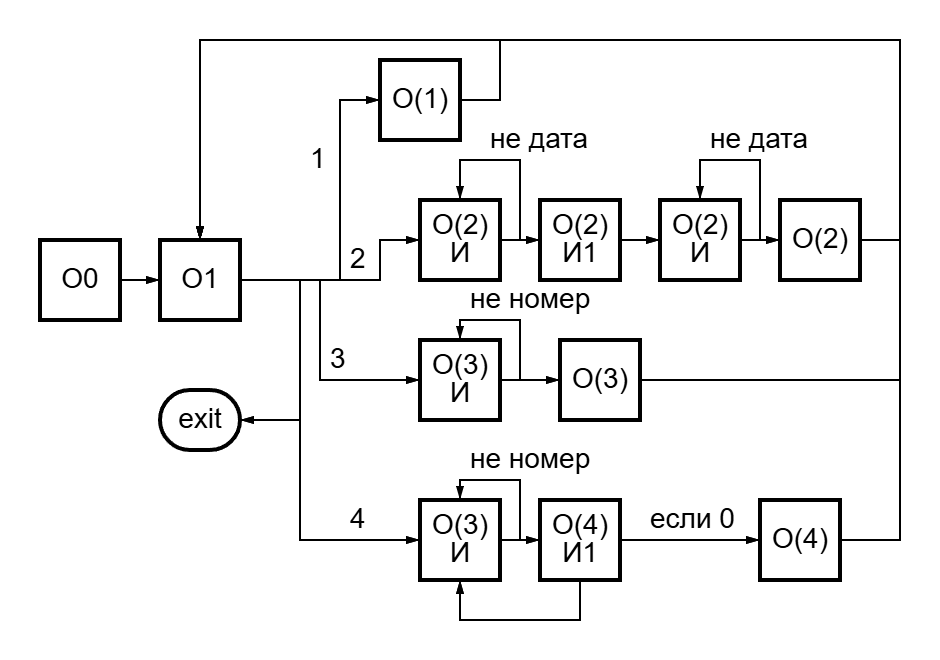
\includegraphics[width=0.7\linewidth]{pics/inputs_diagram.png}
\end{center}

o(1).txt:
\lstinputlisting{files/os_templates/o(1).txt}

o(2).txt:
\lstinputlisting{files/os_templates/o(2).txt}

o(2)i.txt:
\lstinputlisting{files/os_templates/o(2)i.txt}

o(2)i1.txt:
\lstinputlisting{files/os_templates/o(2)i1.txt}

o(3).txt:
\lstinputlisting{files/os_templates/o(3).txt}

o(3)i.txt:
\lstinputlisting{files/os_templates/o(3)i.txt}

o(4).txt:
\lstinputlisting{files/os_templates/o(4).txt}

O(4)i.txt:
\lstinputlisting{files/os_templates/O(4)i.txt}

o0.txt:
\lstinputlisting{files/os_templates/o0.txt}

o1.txt:
\lstinputlisting{files/os_templates/o1.txt}

task.txt:
\lstinputlisting{files/os_templates/task.txt}

\section{Работа с файлами}
Шаблон файла ввода исполнителей:
{
    \ttfamily
    \{number\}|\{name\}|\{address\}
}

Шаблон файла ввода задач:
{
    \ttfamily
    \{name\}|\{rate\}|\{fee\}|\{scope\}|\{date\}|\{executors\} ИЛИ

    \{name\}|\{rate\}|\{fee\}\$||\{executors\}
}

\section{Реализация ввода/вывода}
Ввод команд производится в консоли с помнощью потока std::cin и вывода результата в
потоки std::cout и std::ostream.

\section{Внутреннее представление данных и описание структур}
\begin{center}
    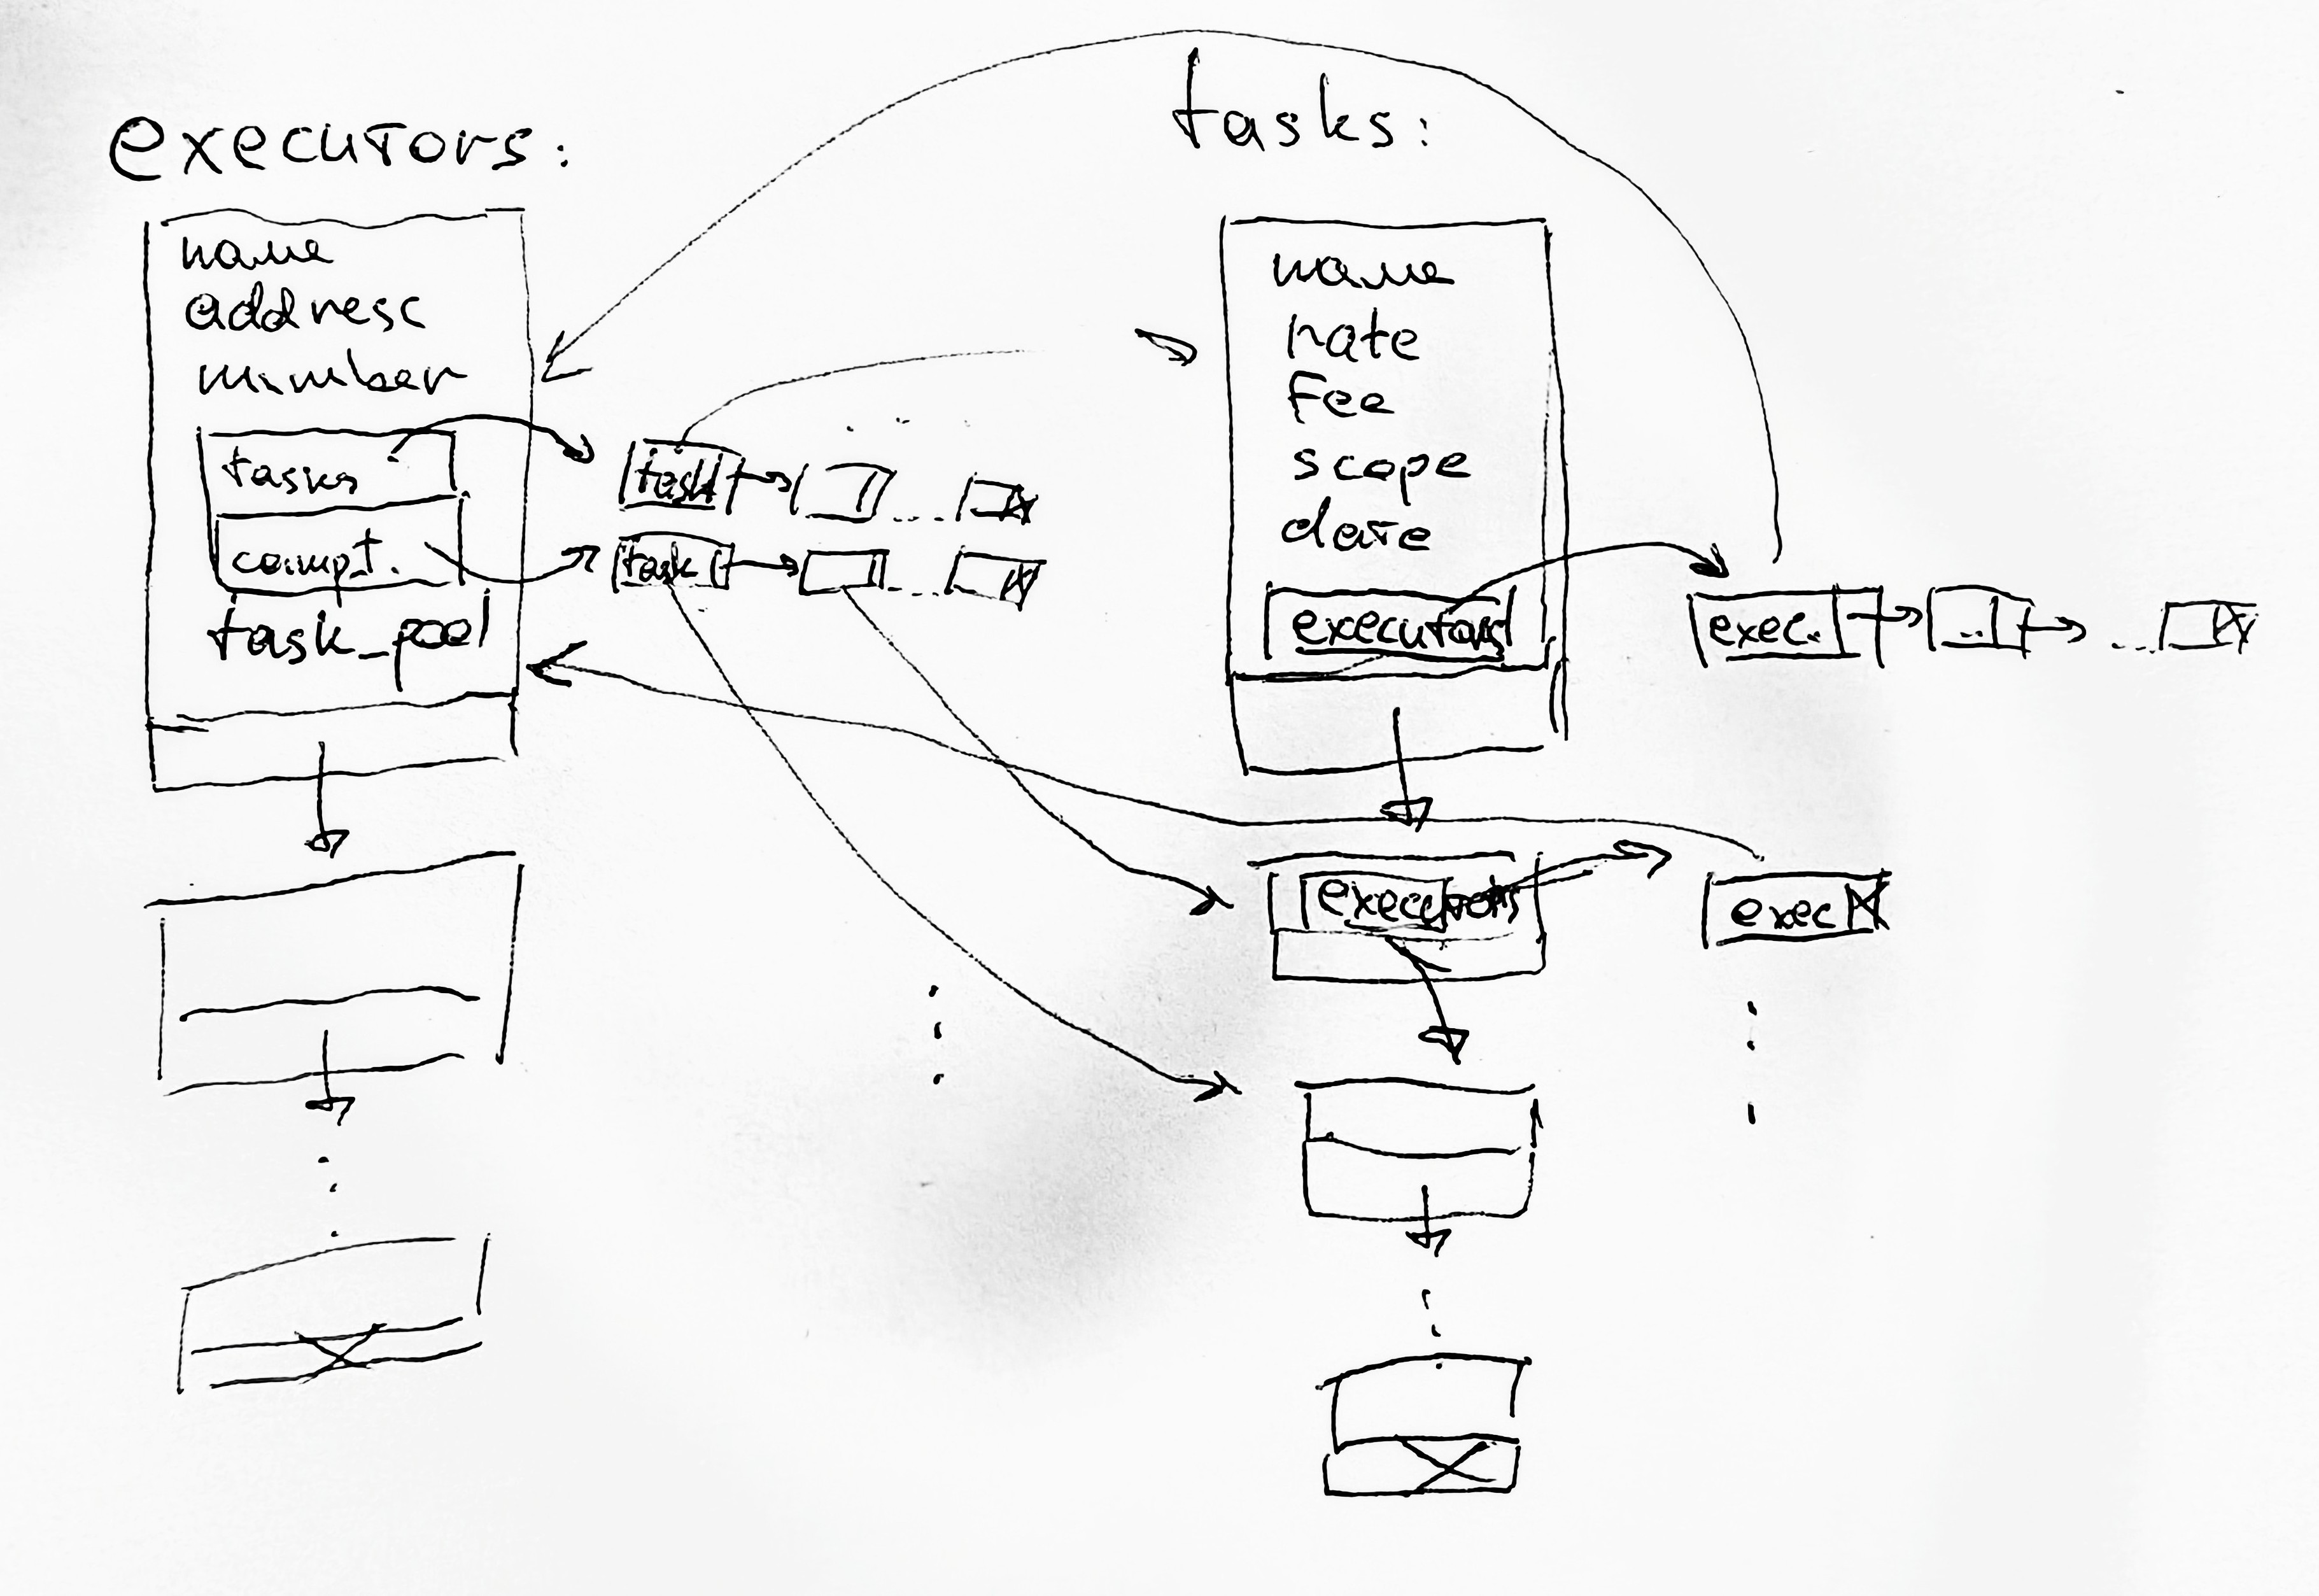
\includegraphics[width=0.7\linewidth]{pics/IMG_20250522_135526_725.jpg}
\end{center}

Переменные главного потока

\begin{xltabular}{\textwidth}{|
>{\hsize=.2\hsize\centering\arraybackslash\ttfamily\bfseries}X|
>{\hsize=.2\hsize\centering\arraybackslash\itshape}X|
>{\hsize=.6\hsize\centering\arraybackslash}X|
}
\hline
\multicolumn{1}{|>{\hsize=.2\hsize\centering\arraybackslash}X}{Имя переменной} &
\multicolumn{1}{|>{\hsize=.2\hsize\centering\arraybackslash}X}{Тип} &
\multicolumn{1}{|>{\hsize=.6\hsize\centering\arraybackslash}X|}{Описание} \\ \hline
in\_exec, in\_tasks & ifstream & Входные файлы списков \\ \hline
tasks & list<Task> & Общий список задач \\ \hline
executors & list<Executor> & Общий список исполнителей \\ \hline
tasks\_pool & MultiTask & Пул задач \\ \hline
\end{xltabular}

Структура {\ttfamily\bfseries list} (из {\ttfamily abstracts.hpp}):

Абстракция, шаблон. Список для всех всех списков. Используется много где, унифицирован.
\begin{xltabular}{\textwidth}{|
    >{\hsize=.2\hsize\centering\arraybackslash\ttfamily\bfseries}X|
    >{\hsize=.2\hsize\centering\arraybackslash\itshape}X|
    >{\hsize=.6\hsize\centering\arraybackslash}X|
    }
    \hline
    \multicolumn{1}{|>{\hsize=.2\hsize\centering\arraybackslash}X}{Имя переменной} &
    \multicolumn{1}{|>{\hsize=.2\hsize\centering\arraybackslash}X}{Тип} &
    \multicolumn{1}{|>{\hsize=.6\hsize\centering\arraybackslash}X|}{Описание} \\ \hline
    is\_virtual & bool & Флаг "виртуальности" списка \\ \hline
    first, last & Node* & Первый и последний ноды \\ \hline
    spec\_bytes & char[sizeof(SpecT)] & Специфические байты информации \\ \hline
\end{xltabular}

Структура {\ttfamily\bfseries list::Node} (из {\ttfamily abstracts.hpp}):

Абстракция, кусок внутри шаблона. Нод всех нодов. Используется много где, унифицирован.
\begin{xltabular}{\textwidth}{|
>{\hsize=.2\hsize\centering\arraybackslash\ttfamily\bfseries}X|
>{\hsize=.2\hsize\centering\arraybackslash\itshape}X|
>{\hsize=.6\hsize\centering\arraybackslash}X|
}
\hline
\multicolumn{1}{|>{\hsize=.2\hsize\centering\arraybackslash}X}{Имя переменной} &
\multicolumn{1}{|>{\hsize=.2\hsize\centering\arraybackslash}X}{Тип} &
\multicolumn{1}{|>{\hsize=.6\hsize\centering\arraybackslash}X|}{Описание} \\ \hline
value & V* & Указатель на значение узла \\ \hline
next & Node* & Указатель на следующий узел в списке \\ \hline
\end{xltabular}

Структура {\ttfamily\bfseries date} (из {\ttfamily types.hpp}):

Хранит дату в 3 байтах, жесть. Очень много битовой магии и масок.
\begin{xltabular}{\textwidth}{|
    >{\hsize=.2\hsize\centering\arraybackslash\ttfamily\bfseries}X|
    >{\hsize=.2\hsize\centering\arraybackslash\itshape}X|
    >{\hsize=.6\hsize\centering\arraybackslash}X|
    }
    \hline
    \multicolumn{1}{|>{\hsize=.2\hsize\centering\arraybackslash}X}{Имя переменной} &
    \multicolumn{1}{|>{\hsize=.2\hsize\centering\arraybackslash}X}{Тип} &
    \multicolumn{1}{|>{\hsize=.6\hsize\centering\arraybackslash}X|}{Описание} \\ \hline
    bytes & unsigned char[3] & байты информации о дате \\ \hline
\end{xltabular}


Структура {\ttfamily\bfseries StrChunk} (из {\ttfamily types.hpp}):

Куски строки. Статической длинны. Унифицированы для использования в качестве значения нода.
\begin{xltabular}{\textwidth}{|
>{\hsize=.2\hsize\centering\arraybackslash\ttfamily\bfseries}X|
>{\hsize=.2\hsize\centering\arraybackslash\itshape}X|
>{\hsize=.6\hsize\centering\arraybackslash}X|
}
\hline
\multicolumn{1}{|>{\hsize=.2\hsize\centering\arraybackslash}X}{Имя переменной} &
\multicolumn{1}{|>{\hsize=.2\hsize\centering\arraybackslash}X}{Тип} &
\multicolumn{1}{|>{\hsize=.6\hsize\centering\arraybackslash}X|}{Описание} \\ \hline
s & char[STR\_ CHUNK\_LENGTH] & Буфер для хранения строки (нулевой инициализации) \\ \hline
sep & inline static char[] & Статическая строка разделителя при выводе ( " - > ") \\ \hline
end & inline static char[] & Статическая строка окончания списка ( " - > nullptr") \\ \hline
\end{xltabular}

Структура {\ttfamily\bfseries Task} (из {\ttfamily types.hpp}):

Задачи. Хранят информацию. Унифицированы для использования в качестве значения нода.
\begin{xltabular}{\textwidth}{|
    >{\hsize=.2\hsize\centering\arraybackslash\ttfamily\bfseries}X|
    >{\hsize=.2\hsize\centering\arraybackslash\itshape}X|
>{\hsize=.6\hsize\centering\arraybackslash}X|
}
\hline
\multicolumn{1}{|>{\hsize=.2\hsize\centering\arraybackslash}X}{Имя переменной} &
\multicolumn{1}{|>{\hsize=.2\hsize\centering\arraybackslash}X}{Тип} &
\multicolumn{1}{|>{\hsize=.6\hsize\centering\arraybackslash}X|}{Описание} \\ \hline
name & str & Название задачи \\ \hline
rate & unsigned & Время выполнения (в часах) \\ \hline
fee & unsigned & Стоимость задачи (* 1k рублей) \\ \hline
scope & unsigned & Объем задачи (только для завершенных задач) \\ \hline
completion\_date & date & Дата завершения задачи \\ \hline
executors & list<Executor> & Список исполнителей задачи (виртуальный список) \\ \hline
\_executors \_positions & list<\_Id> & Позиции исполнителей в списке \\ \hline
sep & inline static char[] & Статическая строка разделителя при выводе ("n") \\ \hline
end & inline static char[] & Статическая строка окончания списка ("n") \\ \hline
\end{xltabular}

Структура {\ttfamily\bfseries MultiTask} (из {\ttfamily types.hpp}):

Пул задач. Состоит из 2 списков. Виртуальных.
\begin{xltabular}{\textwidth}{|
    >{\hsize=.2\hsize\centering\arraybackslash\ttfamily\bfseries}X|
    >{\hsize=.2\hsize\centering\arraybackslash\itshape}X|
    >{\hsize=.6\hsize\centering\arraybackslash}X|
    }
    \hline
    \multicolumn{1}{|>{\hsize=.2\hsize\centering\arraybackslash}X}{Имя переменной} &
    \multicolumn{1}{|>{\hsize=.2\hsize\centering\arraybackslash}X}{Тип} &
    \multicolumn{1}{|>{\hsize=.6\hsize\centering\arraybackslash}X|}{Описание} \\ \hline
    tasks & list<Task> & Список активных задач \\ \hline
    completed\_tasks & list<Task> & Список выполненных задач \\ \hline
\end{xltabular}

Структура {\ttfamily\bfseries Executor} (из {\ttfamily types.hpp}):

Исполнитель. Хранит адрес исполнителя. Унифицированы для использования в качестве значения нода.
\begin{xltabular}{\textwidth}{|
    >{\hsize=.2\hsize\centering\arraybackslash\ttfamily\bfseries}X|
    >{\hsize=.2\hsize\centering\arraybackslash\itshape}X|
    >{\hsize=.6\hsize\centering\arraybackslash}X|
    }
    \hline
    \multicolumn{1}{|>{\hsize=.2\hsize\centering\arraybackslash}X}{Имя переменной} &
    \multicolumn{1}{|>{\hsize=.2\hsize\centering\arraybackslash}X}{Тип} &
    \multicolumn{1}{|>{\hsize=.6\hsize\centering\arraybackslash}X|}{Описание} \\ \hline
    service\_number & unsigned long & Уникальный номер исполнителя \\ \hline
    name & str & Имя исполнителя \\ \hline
    address & str & Адрес исполнителя \\ \hline
    task\_pool & MultiTask & Пул задач исполнителя \\ \hline
    sep & inline static char[] & Статическая строка разделителя при выводе ("n") \\ \hline
    end & inline static char[] & Статическая строка окончания списка ("n") \\ \hline
\end{xltabular}


\section{Модульное представление программы}

\begin{center}
    
\includegraphics[width=0.7\linewidth]{pics/module_diagram.png}
\end{center}

\section{Описание алгоритма}
Описание работы списка было опущено (см. предыдущие ЛР). 

\subsection{Считывание (file)}
Считывание производится с помощью перегрузки оператора > >. Для каждого типа
(включая строку) прописана данная перегрузка.

\begin{center}\textbf{Перегрузка оператора >> для класса str}\end{center}
\begin{center}
    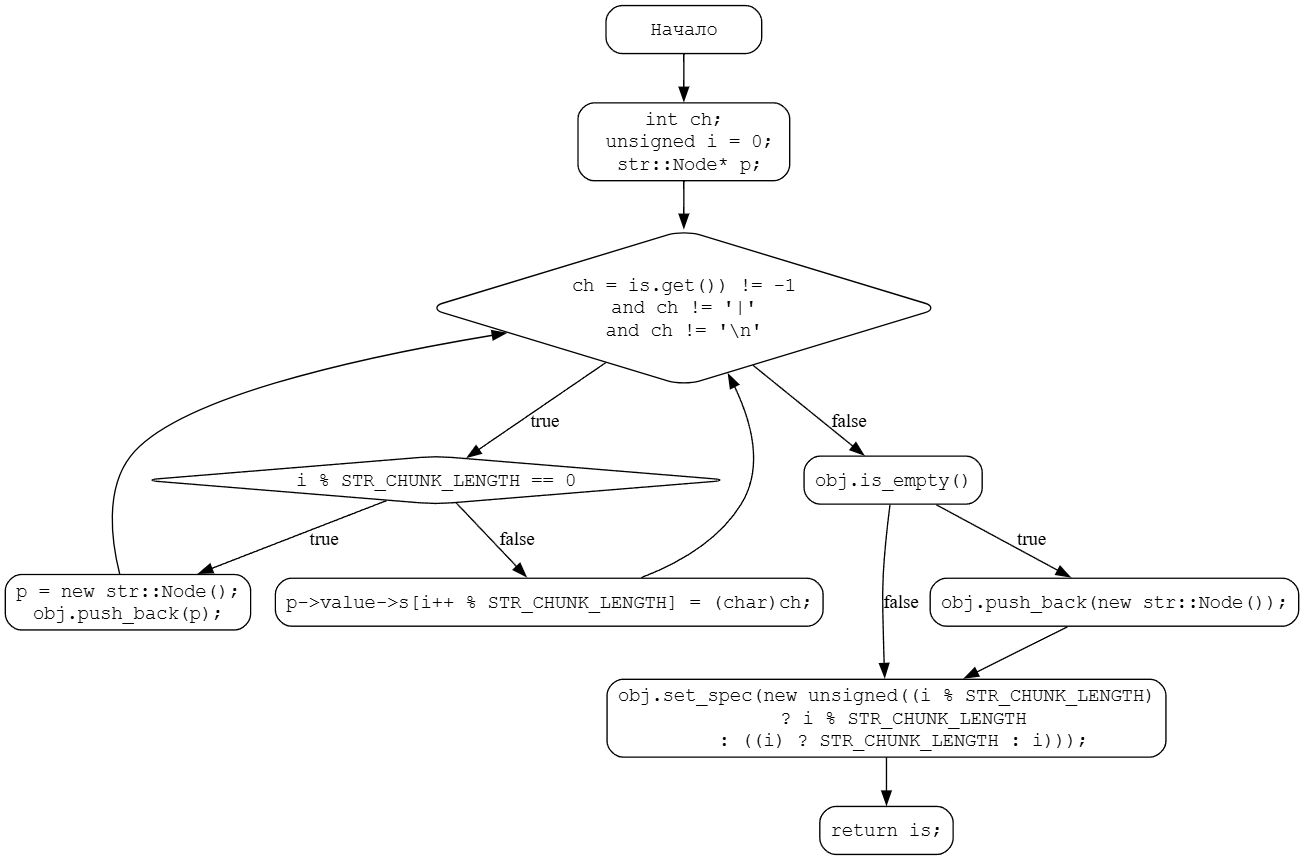
\includegraphics[width=0.8\linewidth]{pics/input_str.png}
\end{center}
\textbf{Краткое описание:} \\
Читает строку из входного потока \texttt{istream}, пока не встретит символ '|' или '\textbackslash n'. Считанные символы сохраняются в объекте класса \texttt{str}, который состоит из цепочки узлов (\texttt{Node}), каждый из которых содержит фиксированное количество символов (STR\_CHUNK\_LENGTH). Также устанавливается спецификация длины последнего блока.


\textbf{Параметры:}


- \texttt{istream\& is} — входной поток. (\textit{входной})

- \texttt{str\& obj} — объект класса \texttt{str}, в который записываются считанные данные. (\textit{изменяемый})

\begin{center}\textbf{Перегрузка оператора >> для класса Executor}\end{center}
\begin{center}
    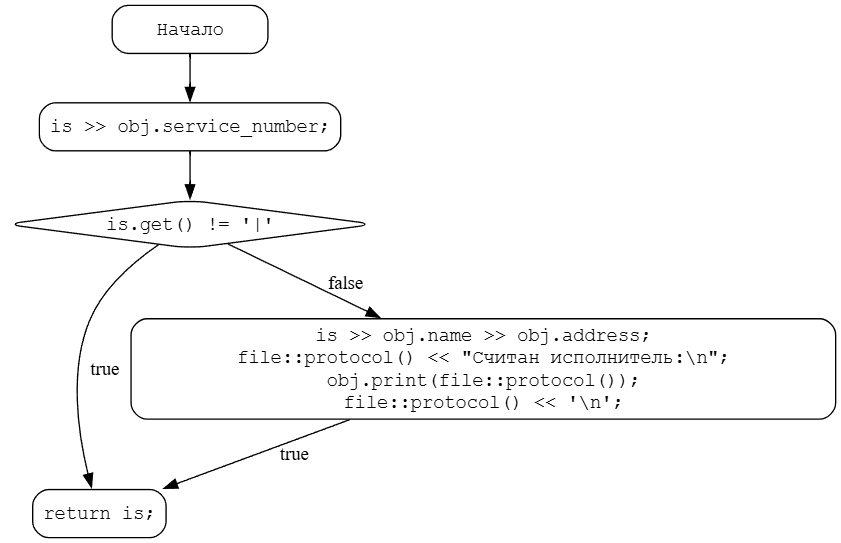
\includegraphics[width=0.7\textwidth]{pics/input_executor.png}
\end{center}
\textbf{Краткое описание:} \\
Считывает поля объекта класса \texttt{Executor}: номер услуги, имя и адрес, разделяемые символом '|'. После чтения выводит информацию в протокол с помощью \texttt{file::protocol()}.

\textbf{Параметры:}


- \texttt{istream\& is} — входной поток. (\textit{входной})

- \texttt{Executor\& obj} — объект класса \texttt{Executor}, в который записываются считанные данные. (\textit{изменяемый})


\begin{center}\textbf{Перегрузка оператора >> для list$<$\_Id$>$}\end{center}

\textbf{Краткое описание:} \\
Считывает последовательность чисел, представляющих идентификаторы, из входного потока до тех пор, пока встречаются пробелы. Каждый идентификатор добавляется в список \texttt{list$<$\_Id$>$} как новый элемент.

\textbf{Параметры:}


- \texttt{istream\& is} — входной поток. (\textit{входной})

- \texttt{list$<$\_Id$>$\& obj} — список идентификаторов, в который добавляются новые элементы. (\textit{изменяемый})


\begin{center}\textbf{Перегрузка оператора >> для класса Task}\end{center}
\textbf{Краткое описание:} \\
Считывает поля задачи (\texttt{name}, \texttt{rate}, \texttt{fee}, \texttt{scope}, \texttt{completion\_date}, \texttt{\_executors\_positions}) из входного потока. Используются разделители '|', '\$' и пробелы. После чтения информация записывается в протокол.

\textbf{Параметры:}


- \texttt{istream\& is} — входной поток. (\textit{входной})

- \texttt{Task\& obj} — объект класса \texttt{Task}, в который записываются считанные данные. (\textit{изменяемый})
\begin{center}
    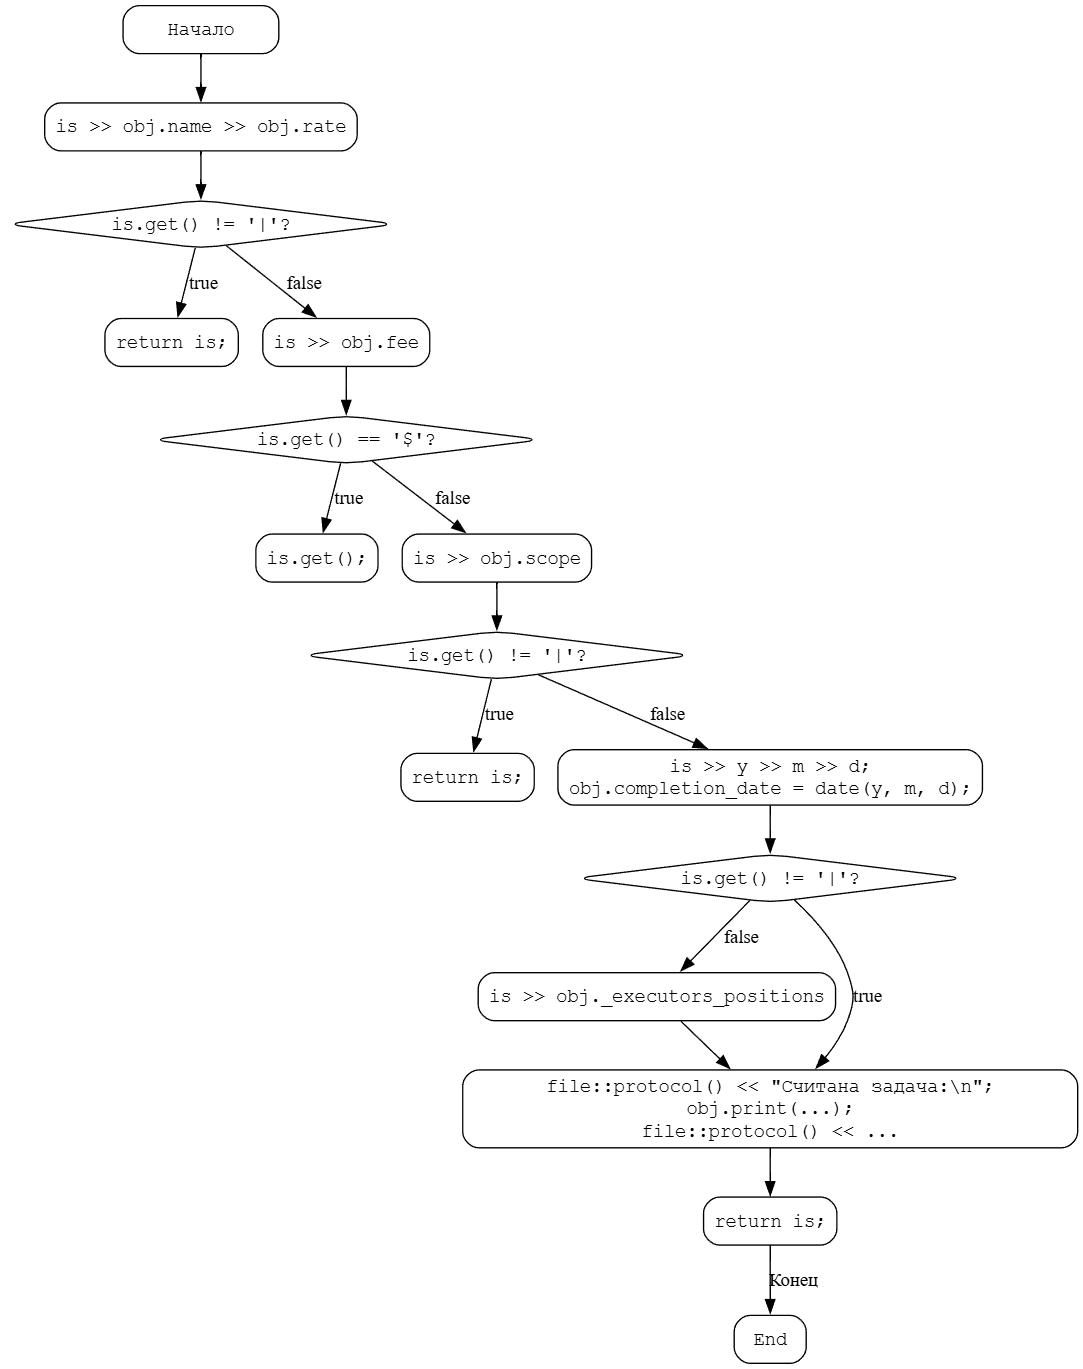
\includegraphics[width=0.7\textwidth]{pics/input_task.png}
\end{center}

\begin{center}
    \textbf{перегрузка оператора >> для класса date}
\end{center}
\textbf{Краткое описание:} \\
Считывает дату в виде трёх чисел: год (unsigned), месяц (short unsigned), день (short unsigned). Создаёт временный объект \texttt{date}, а затем копирует его внутреннее представление (\texttt{bytes}) в целевой объект.

\textbf{Параметры:}


- \texttt{istream\& is} — входной поток. (\textit{входной})

- \texttt{date\& obj} — объект класса \texttt{date}, в который записывается дата. (\textit{изменяемый})



\subsection{Линкование (linking)}
\begin{center}
    \textbf{Функция: \texttt{add\_to\_multitask(MultiTask* mt, Task* t\_ptr)}}

\end{center}

Краткое описание: \\
Добавляет задачу в один из двух списков объекта \texttt{MultiTask}: \texttt{tasks}, если дата завершения пустая, или \texttt{completed\_tasks}, если дата указана.

Параметры:


- \texttt{MultiTask* mt} — указатель на объект класса \texttt{MultiTask}. (\textit{изменяемый})

- \texttt{Task* t\_ptr} — указатель на объект класса \texttt{Task}. (\textit{входной})

\begin{center}
    \textbf{Функция: \texttt{fill\_multitask(MultiTask* mt, list<Task>\& ts)}}

\end{center}

Краткое описание: \\
Переносит все задачи из списка \texttt{ts} в соответствующие списки объекта \texttt{MultiTask}, используя функцию \texttt{add\_to\_multitask} для каждой задачи.

Параметры:


- \texttt{MultiTask* mt} — указатель на объект класса \texttt{MultiTask}. (\textit{изменяемый})

- \texttt{list<Task>\& ts} — ссылка на список задач. (\textit{входной})

\begin{center}
    \textbf{Функция: \texttt{form\_bond(ExecutorN* e\_ptr, TaskN* t\_ptr)}}

\end{center}

Краткое описание: \\
Устанавливает двустороннюю связь между исполнителем и задачей: добавляет задачу в пул задач исполнителя и добавляет копию узла исполнителя в список исполнителей задачи.

Параметры:


- \texttt{ExecutorN* e\_ptr} — указатель на узел списка исполнителей. (\textit{входной})

- \texttt{TaskN* t\_ptr} — указатель на узел списка задач. (\textit{изменяемый})

\begin{center}
    \textbf{Функция: \texttt{link\_executors\_to\_tasks(list<Executor>\& es, list<Task>\& ts)}}
    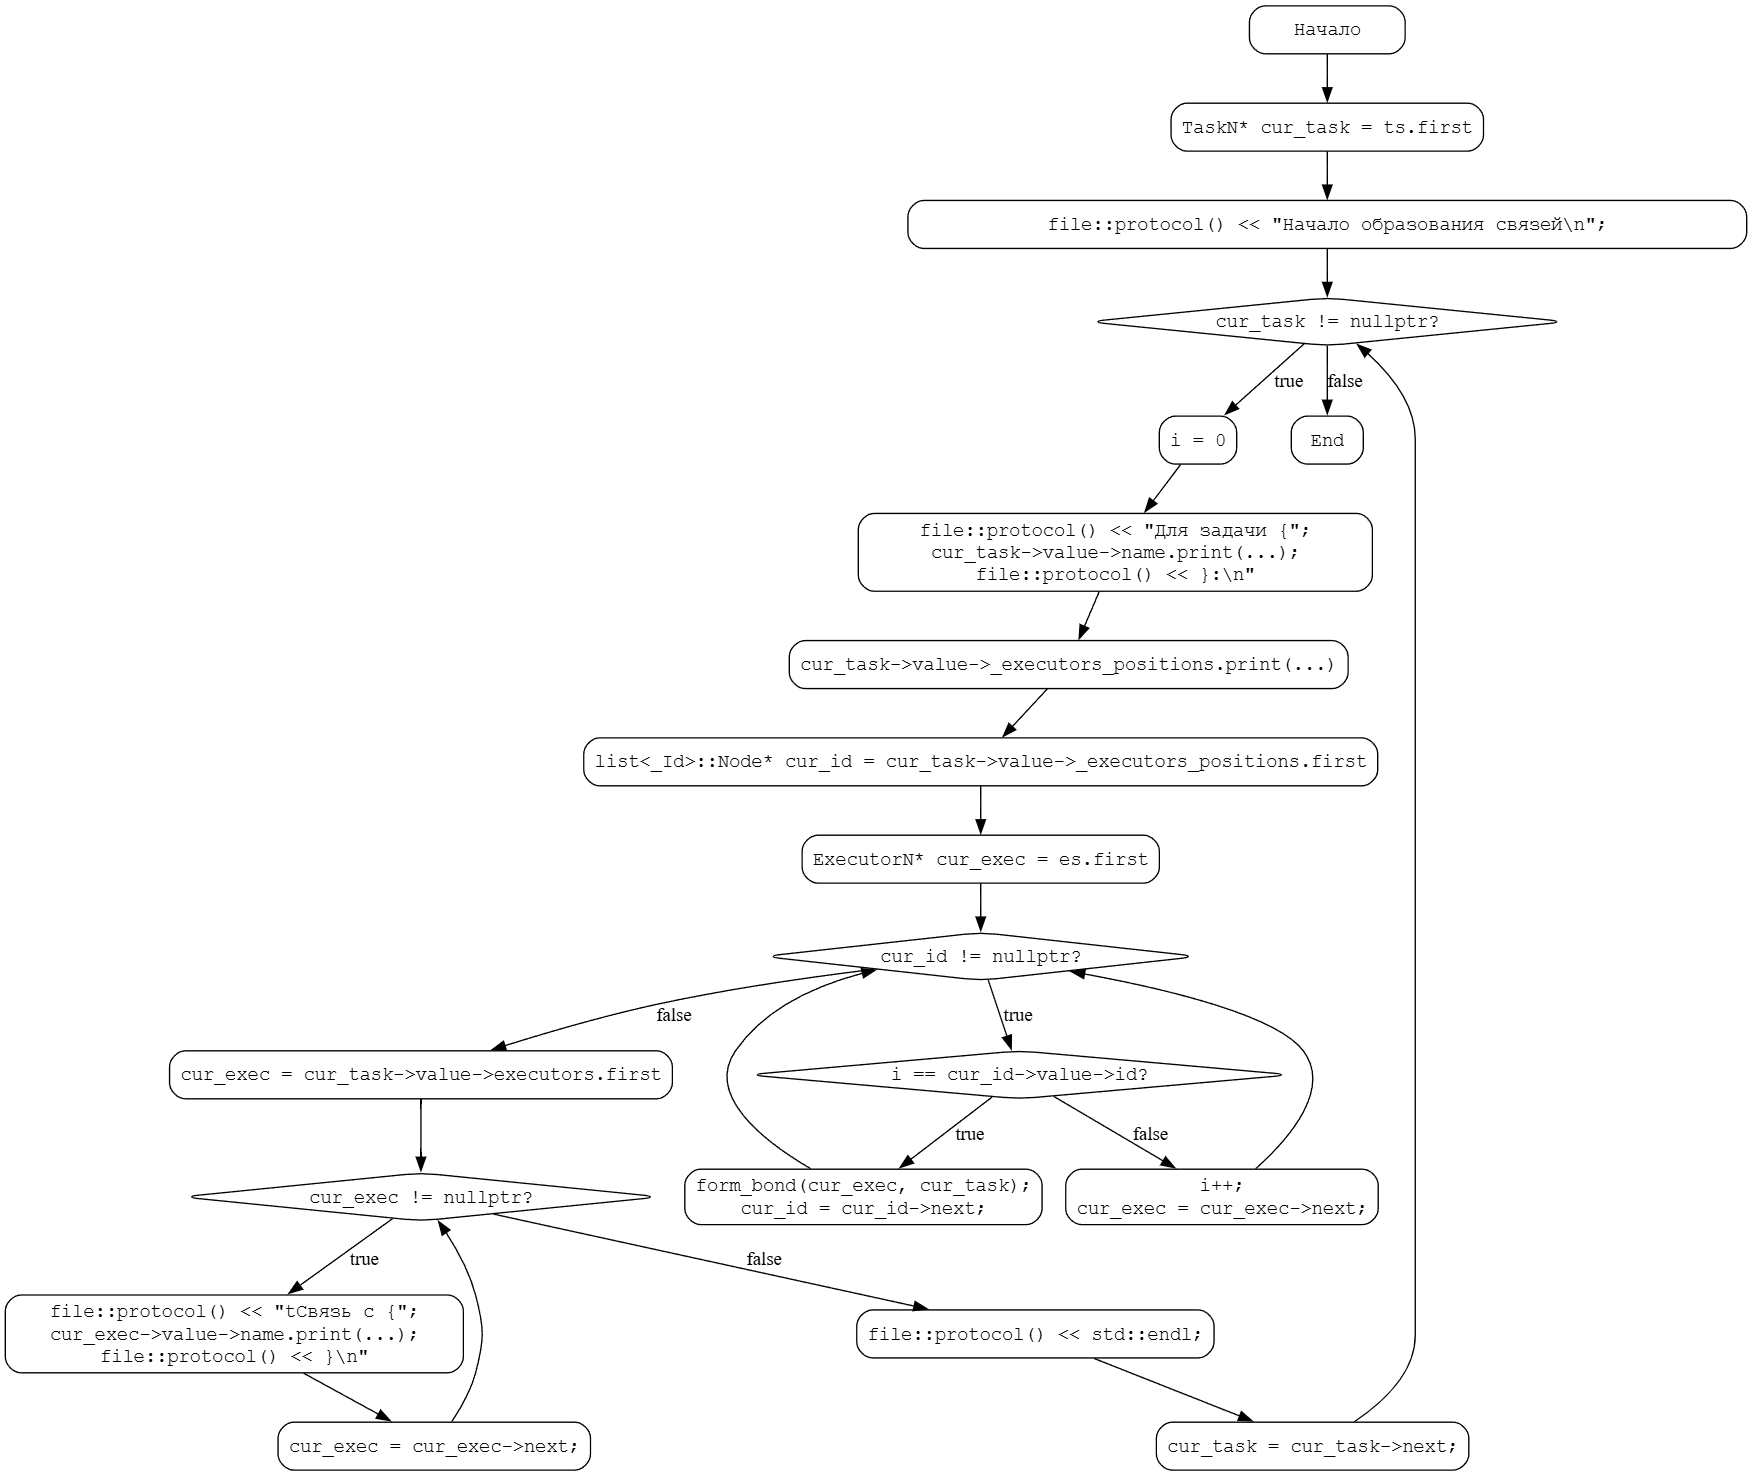
\includegraphics[width=\linewidth]{pics/linking_link.png}
\end{center}

Краткое описание: \\
Создаёт связи между исполнителями и задачами на основе списка идентификаторов исполнителей, хранящегося в каждой задаче. Для каждой задачи находятся соответствующие исполнители по индексам, вызывается функция \texttt{form\_bond}, а результат записывается в протокол.

Параметры:


- \texttt{list<Executor>\& es} — ссылка на список исполнителей. (\textit{входной})

- \texttt{list<Task>\& ts} — ссылка на список задач. (\textit{входной})

\subsection{Вывод (menu)}
\begin{center}
    \textbf{Функция: \texttt{loop\_main(std::istream \&is, std::ostream \&os, list<Task>\& tasks, list<Executor>\& executors, MultiTask \&tasks\_pool)}}
    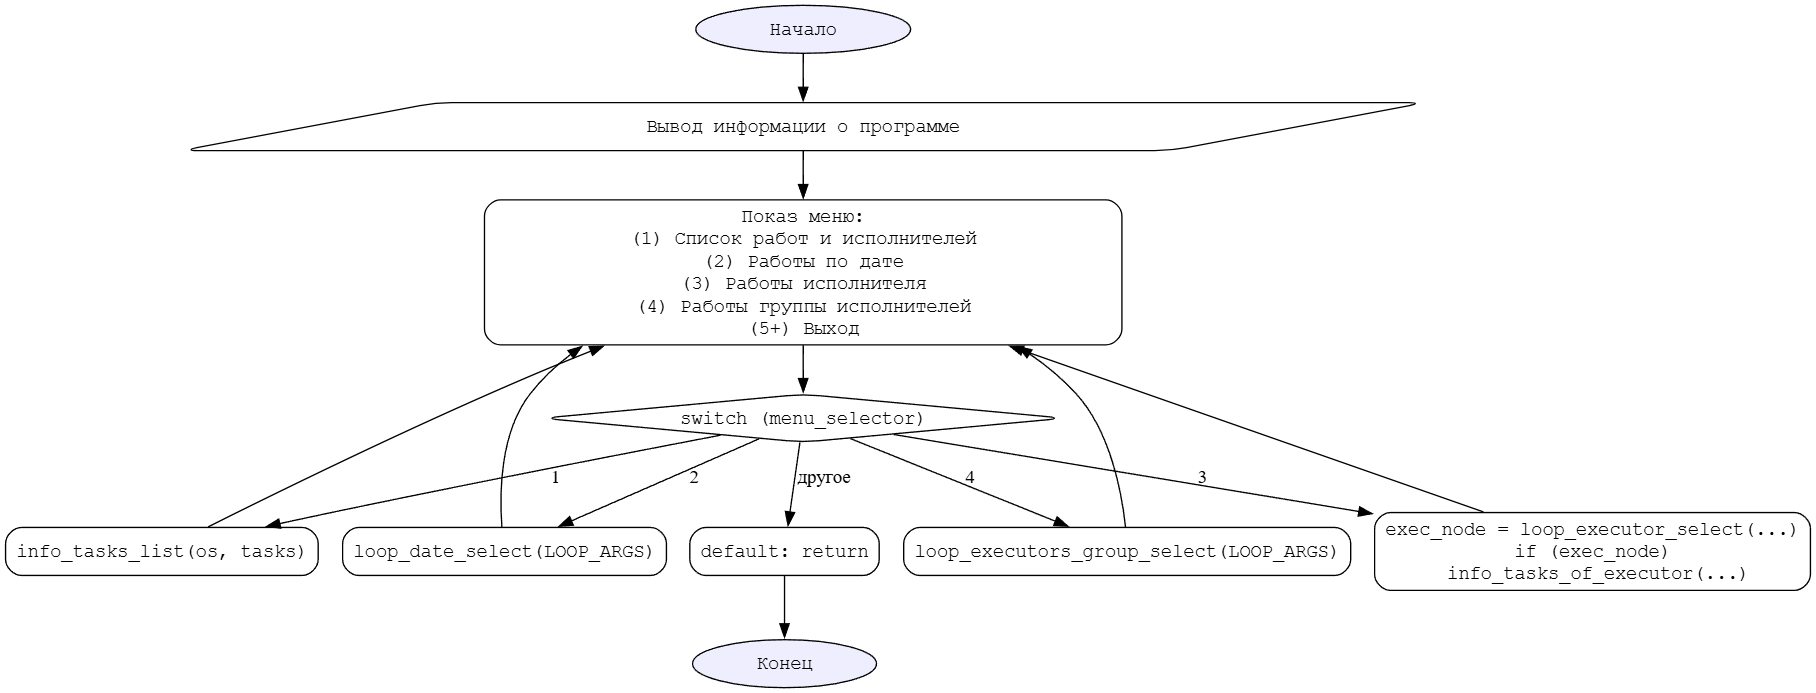
\includegraphics[width=\linewidth]{pics/menu_main.png}
\end{center}

Краткое описание: \\
Основная функция цикла взаимодействия с пользователем. Обрабатывает команды, предоставляет меню, вызывает другие функции для выполнения действий над задачами и исполнителями.

Параметры:


- \texttt{std::istream\& is} — входной поток для чтения команд пользователя. (\textit{входной})

- \texttt{std::ostream\& os} — выходной поток для вывода информации. (\textit{выходной})

- \texttt{list<Task>\& tasks} — ссылка на список задач. (\textit{изменяемый})

- \texttt{list<Executor>\& executors} — ссылка на список исполнителей. (\textit{изменяемый})

- \texttt{MultiTask\& tasks\_pool} — объект, содержащий группы задач (активные и завершённые). (\textit{изменяемый})

\begin{center}

    \textbf{Функция: \texttt{info\_tasks\_list(std::ostream \&os, list<Task>\& tasks)}}
\end{center}

Краткое описание: \\
Выводит в указанный поток список задач в человеко-читаемом виде.

Параметры:


- \texttt{std::ostream\& os} — выходной поток для вывода информации. (\textit{выходной})

- \texttt{list<Task>\& tasks} — ссылка на список задач для вывода. (\textit{входной})

\begin{center}

    \textbf{Функция: \texttt{loop\_date\_select(LOOP\_ARGS\_DEFINITION)}}
\end{center}

Краткое описание: \\
Обрабатывает команду выборки задач по диапазону дат. Определяет, какие задачи попадают в указанный временной интервал, и выводит информацию о них.

Параметры:


- \texttt{std::istream\& is} — входной поток для чтения дат. (\textit{входной})

- \texttt{std::ostream\& os} — выходной поток для вывода результатов. (\textit{выходной})

- \texttt{list<Task>\& tasks} — ссылка на список задач. (\textit{входной})

- \texttt{list<Executor>\& executors} — ссылка на список исполнителей. (\textit{входной})

- \texttt{MultiTask\& tasks\_pool} — объект, содержащий группы задач. (\textit{входной})

\begin{center}
    \textbf{Функция: \texttt{info\_tasks\_date\_by\_executors(std::ostream \&os, list<Executor>\& executors, date beg, date end)}}
    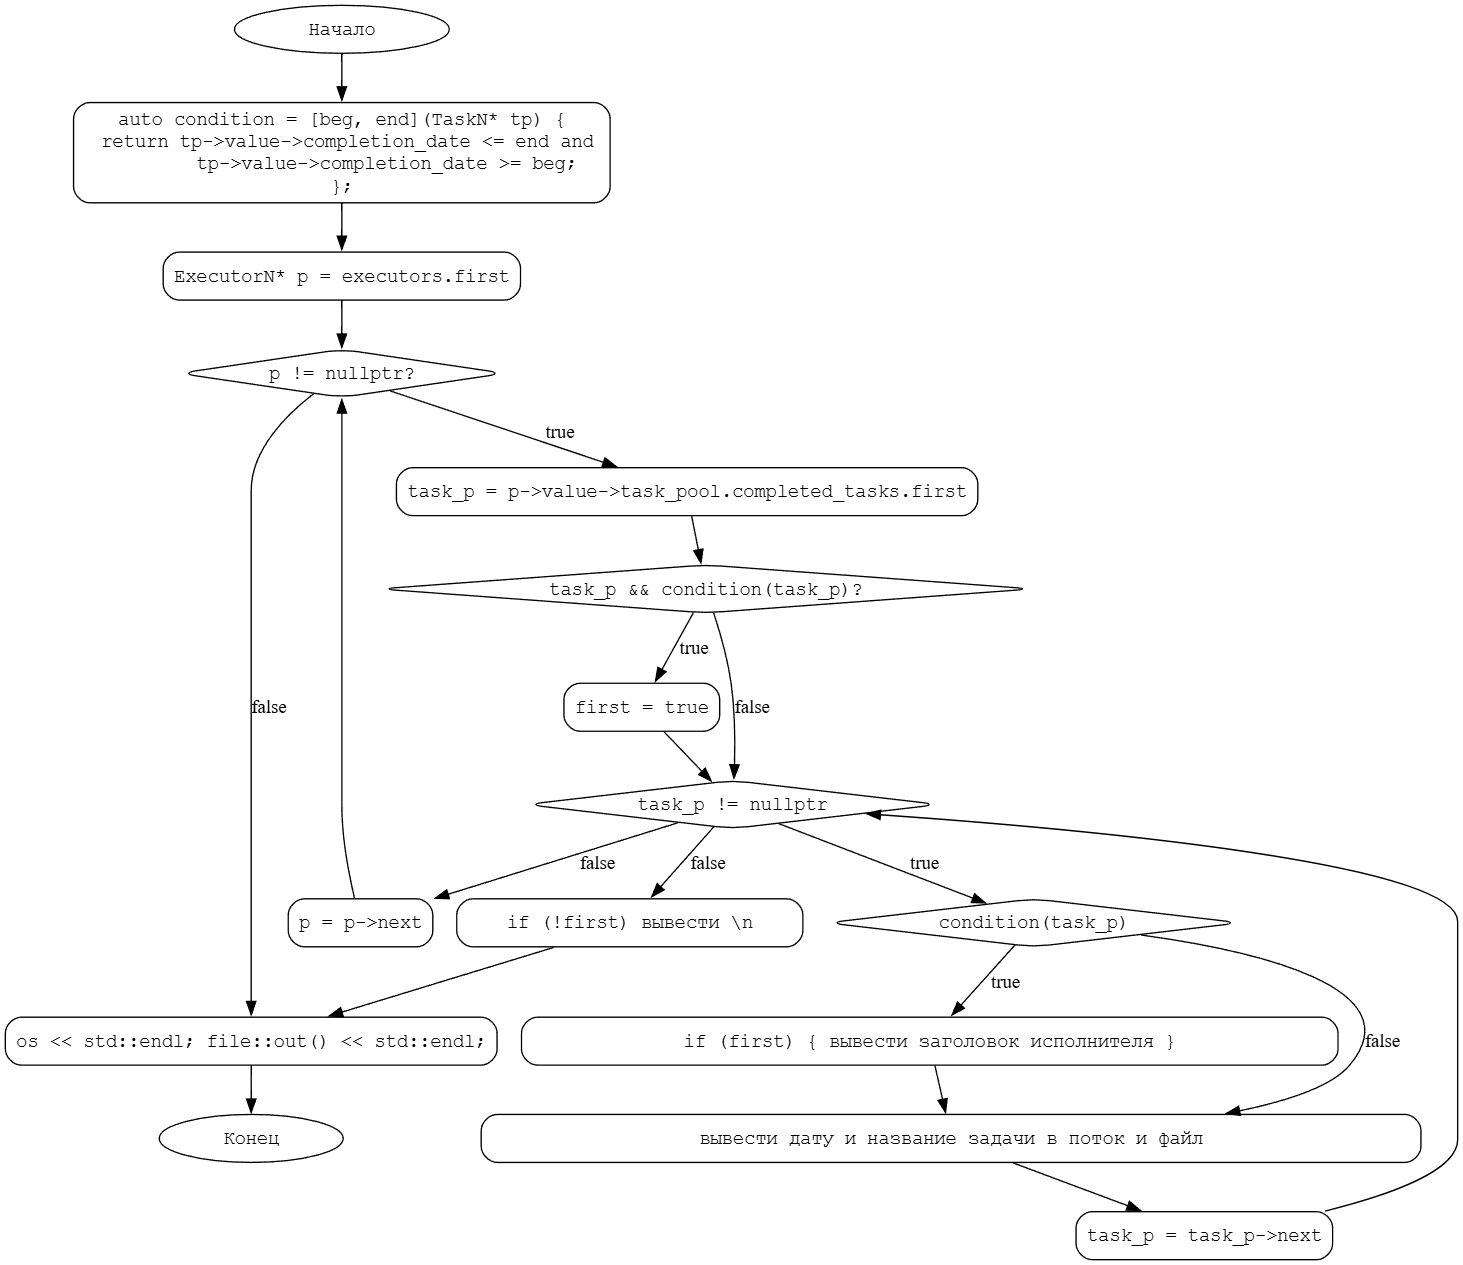
\includegraphics[width=\linewidth]{pics/menu_date_executors.png}
\end{center}

Краткое описание: \\
Выводит информацию о задачах каждого исполнителя, которые попадают в указанный диапазон дат.

Параметры:


- \texttt{std::ostream\& os} — выходной поток для вывода результатов. (\textit{выходной})

- \texttt{list<Executor>\& executors} — ссылка на список исполнителей. (\textit{входной})

- \texttt{date beg} — начало временного интервала. (\textit{входной})

- \texttt{date end} — конец временного интервала. (\textit{входной})

\begin{center}

    \textbf{Функция: \texttt{info\_tasks\_date\_by\_task(std::ostream \&os, list<Task>\& completed\_tasks, date beg, date end)}}
\end{center}

Краткое описание: \\
Выводит информацию о завершённых задачах, попадающих в указанный диапазон дат.

Параметры:


- \texttt{std::ostream\& os} — выходной поток для вывода результатов. (\textit{выходной})

- \texttt{list<Task>\& completed\_tasks} — ссылка на список завершённых задач. (\textit{входной})

- \texttt{date beg} — начало временного интервала. (\textit{входной})

- \texttt{date end} — конец временного интервала. (\textit{входной})

\begin{center}

    \textbf{Функция: \texttt{loop\_executor\_select(LOOP\_ARGS\_DEFINITION)}}
\end{center}

Краткое описание: \\
Выбирает исполнителя из списка для последующего взаимодействия с ним (например, просмотр задач).

Параметры:


- \texttt{std::istream\& is} — входной поток для чтения номера исполнителя. (\textit{входной})

- \texttt{std::ostream\& os} — выходной поток для вывода меню. (\textit{выходной})

- \texttt{list<Task>\& tasks} — ссылка на список задач. (\textit{входной})

- \texttt{list<Executor>\& executors} — ссылка на список исполнителей. (\textit{входной})

- \texttt{MultiTask\& tasks\_pool} — объект, содержащий группы задач. (\textit{входной})

\begin{center}

    \textbf{Функция: \texttt{info\_tasks\_of\_executor(std::ostream \&os, Executor* executor)}}
\end{center}

Краткое описание: \\
Выводит список задач, связанных с конкретным исполнителем.

Параметры:


- \texttt{std::ostream\& os} — выходной поток для вывода информации. (\textit{выходной})

- \texttt{Executor* executor} — указатель на исполнителя, чьи задачи нужно вывести. (\textit{входной})

\begin{center}

    \textbf{Функция: \texttt{loop\_executors\_group\_select(LOOP\_ARGS\_DEFINITION)}}
    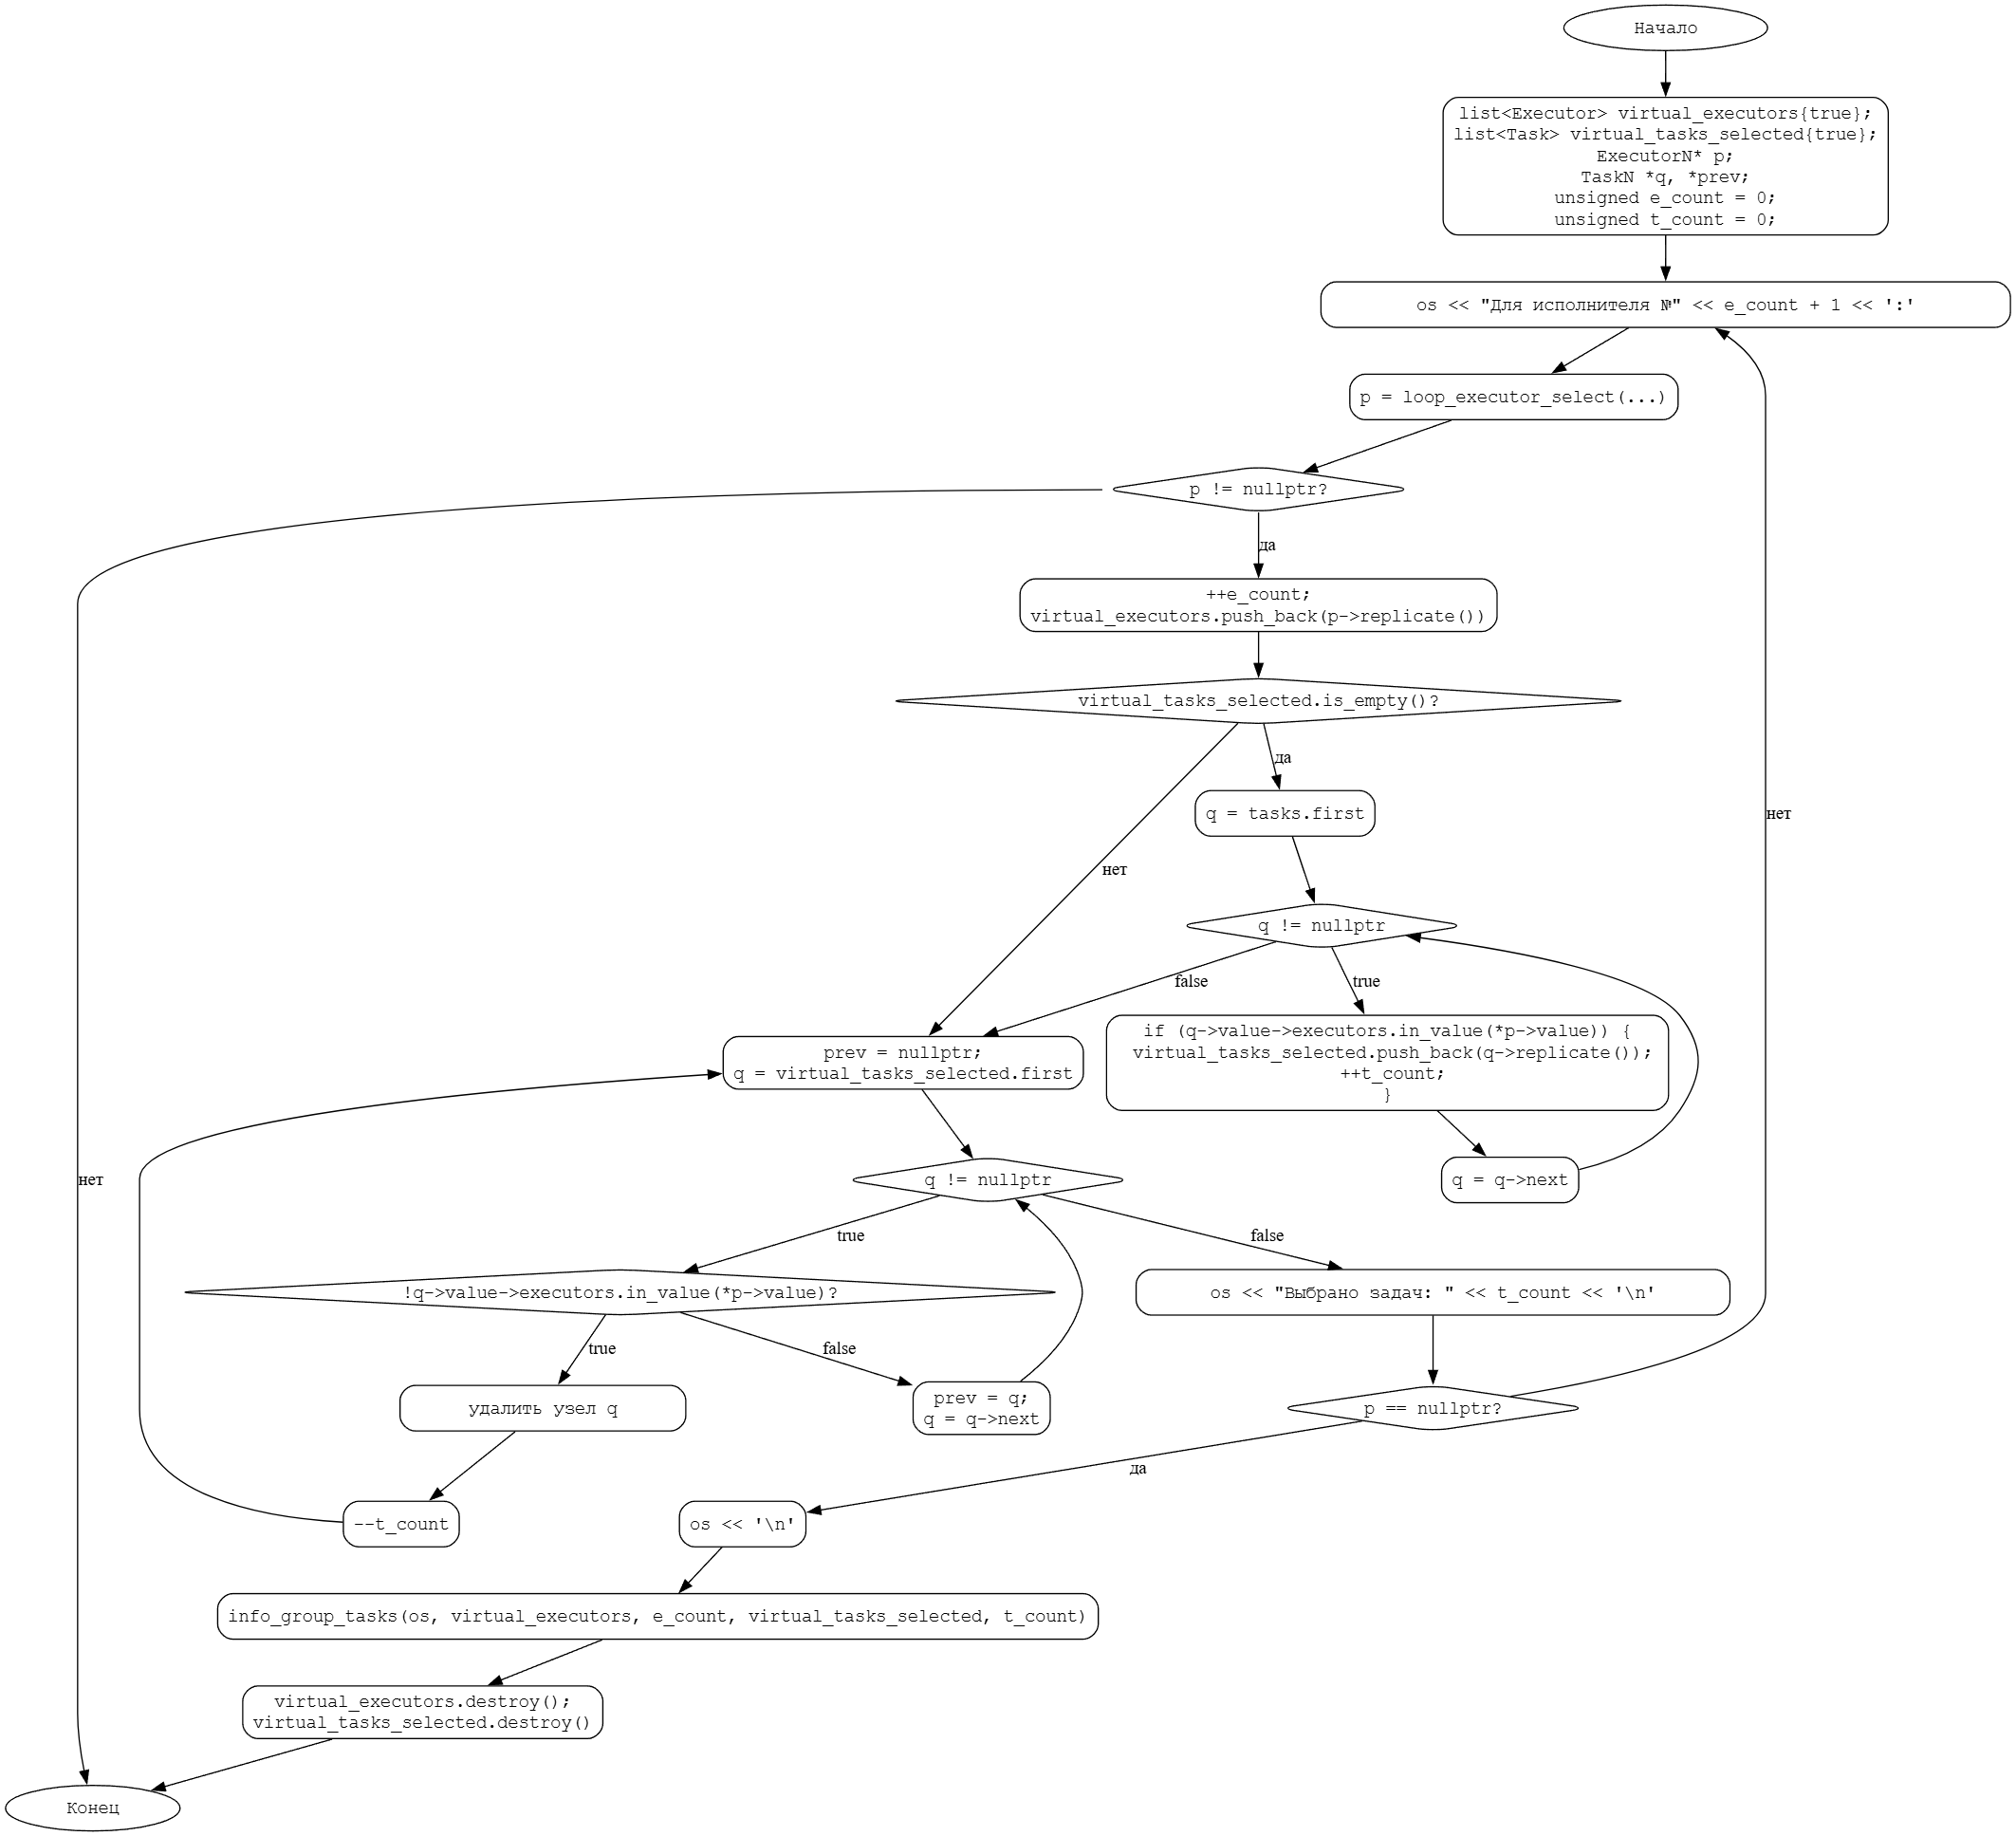
\includegraphics[width=\linewidth]{pics/menu_selector.png}
\end{center}

Краткое описание: \\
Выбирает группу исполнителей и количество задач для вывода, затем вызывает функцию вывода информации о группе.

Параметры:


- \texttt{std::istream\& is} — входной поток для чтения данных от пользователя. (\textit{входной})

- \texttt{std::ostream\& os} — выходной поток для вывода меню и результатов. (\textit{выходной})

- \texttt{list<Task>\& tasks} — ссылка на список задач. (\textit{входной})

- \texttt{list<Executor>\& executors} — ссылка на список исполнителей. (\textit{входной})

- \texttt{MultiTask\& tasks\_pool} — объект, содержащий группы задач. (\textit{входной})

\begin{center}
    \textbf{Функция: \texttt{info\_group\_tasks(std::ostream \&os, list<Executor> executors, unsigned e, list<Task> tasks, unsigned t)}}
    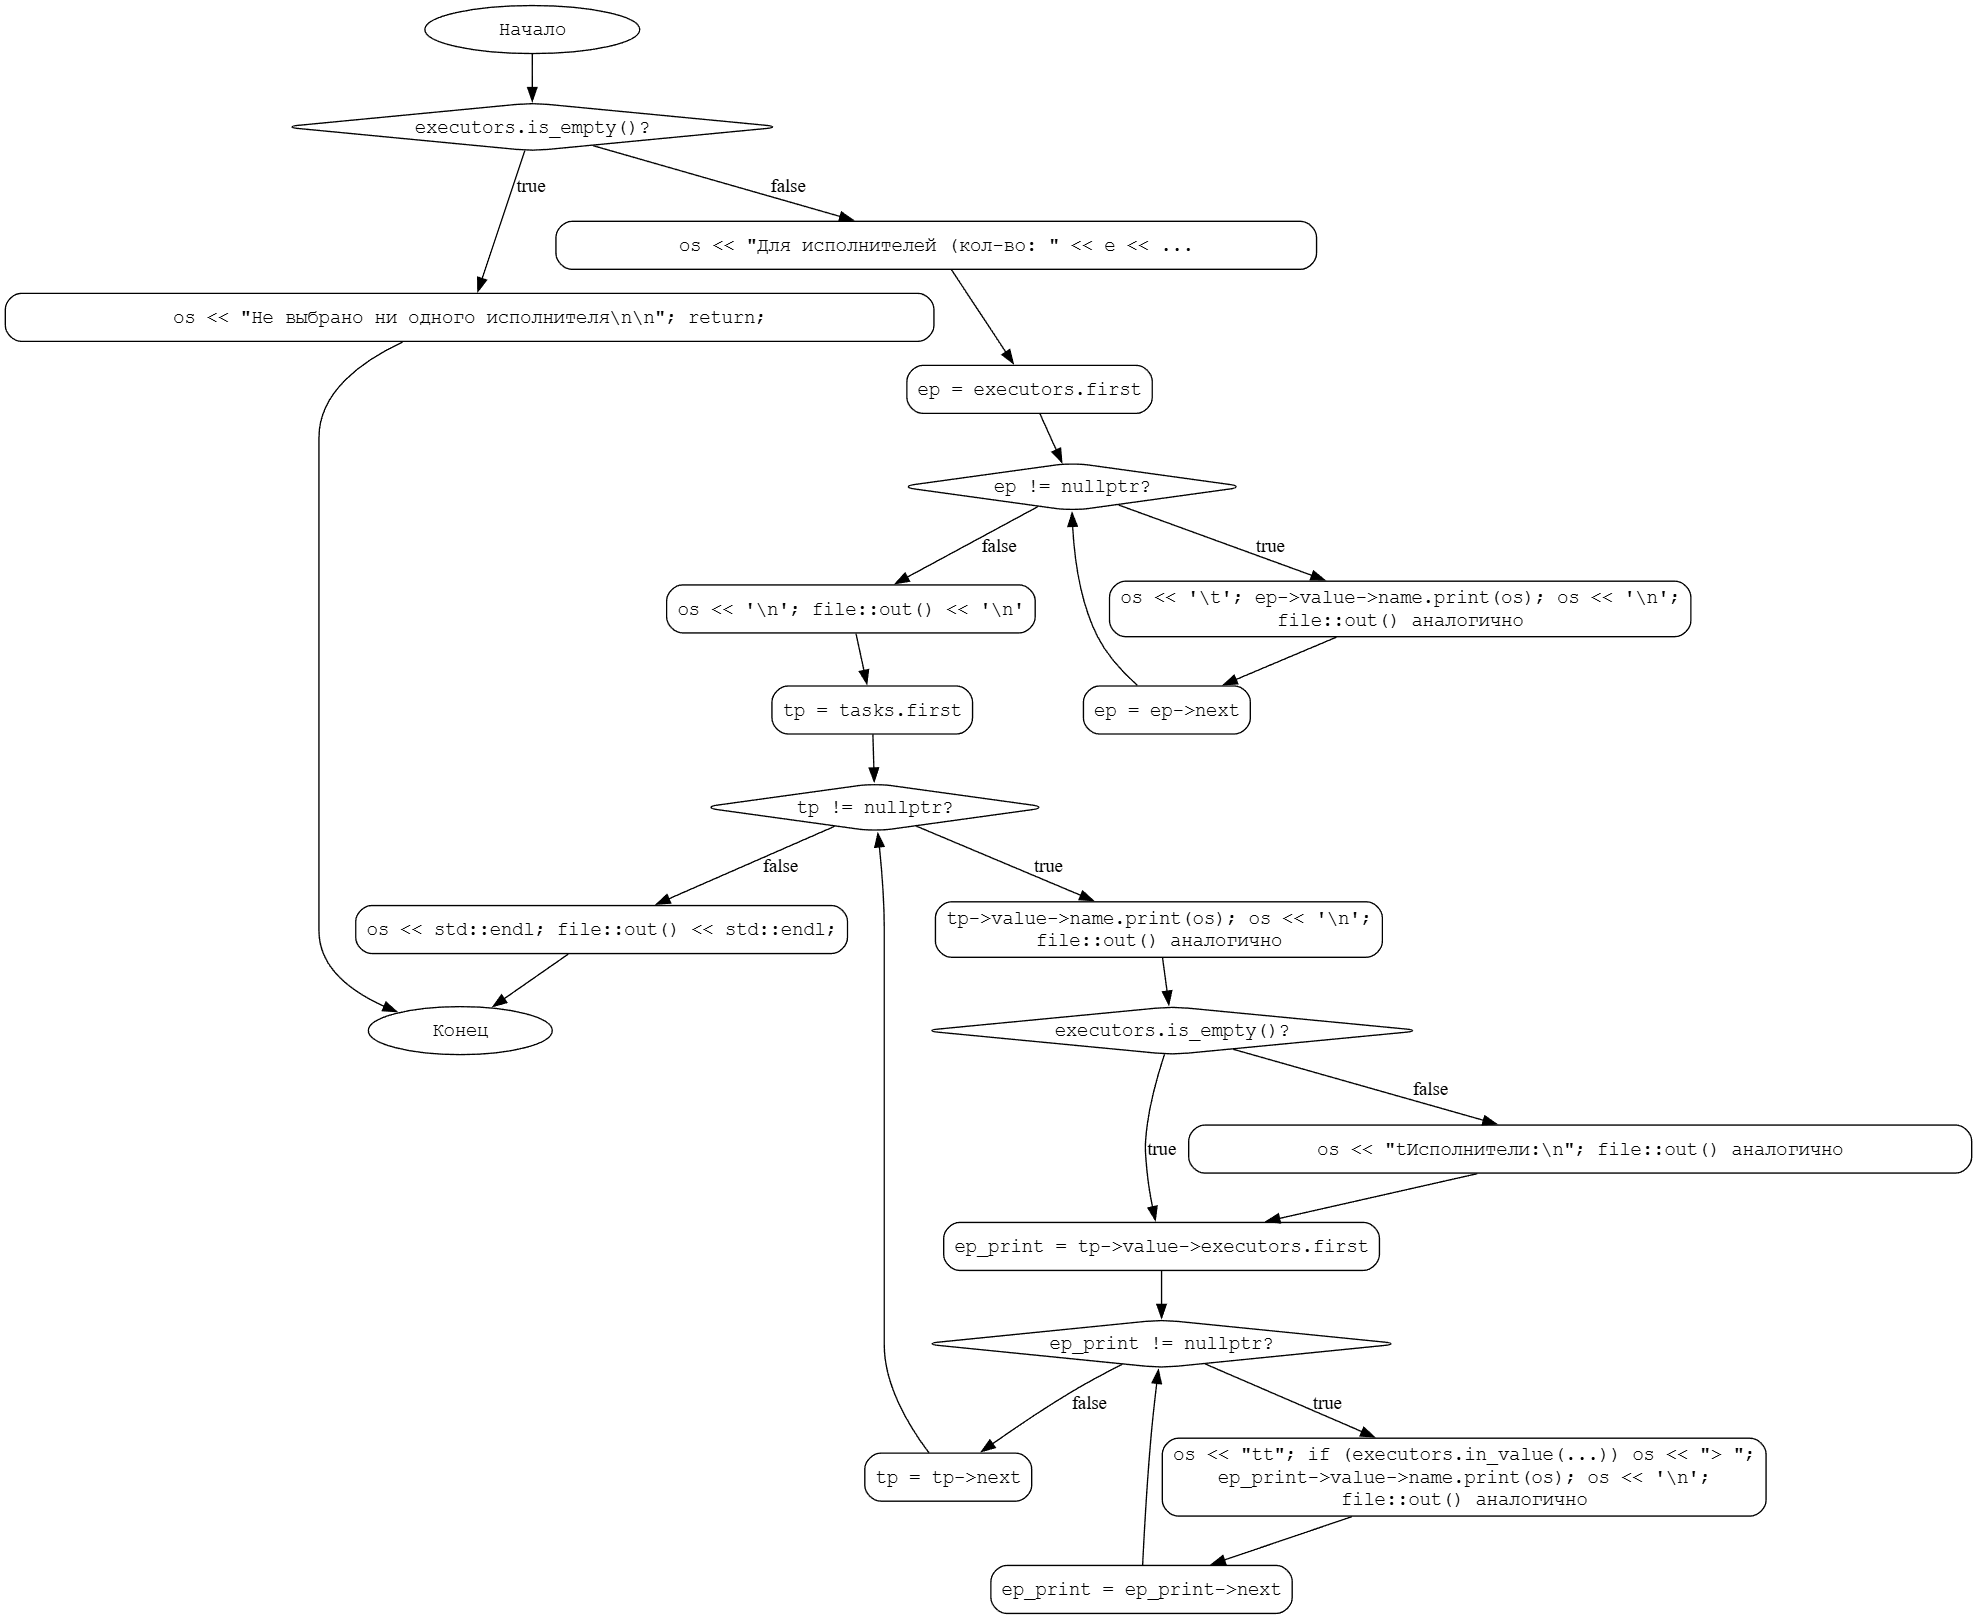
\includegraphics[width=\linewidth]{pics/menu_last_one.png}
\end{center}

Краткое описание: \\
Выводит информацию о заданном количестве исполнителей (\texttt{e}) и связанного с ними заданного числа задач (\texttt{t}).

Параметры:


- \texttt{std::ostream\& os} — выходной поток для вывода информации. (\textit{выходной})

- \texttt{list<Executor> executors} — копия списка исполнителей. (\textit{входной})

- \texttt{unsigned e} — количество исполнителей для вывода. (\textit{входной})

- \texttt{list<Task> tasks} — копия списка задач. (\textit{входной})

- \texttt{unsigned t} — количество задач для вывода. (\textit{входной})

\section{Текст программы}

abstracts.hpp
\lstinputlisting[language=C++]{../../tasks/coursework/abstracts.hpp}
abstracts.ipp
\lstinputlisting[language=C++]{../../tasks/coursework/abstracts.ipp}
const.hpp
\lstinputlisting[language=C++]{../../tasks/coursework/const.hpp}
file.cpp
\lstinputlisting[language=C++]{../../tasks/coursework/file.cpp}
file.hpp
\lstinputlisting[language=C++]{../../tasks/coursework/file.hpp}
file.ipp
\lstinputlisting[language=C++]{../../tasks/coursework/file.ipp}
linking.cpp
\lstinputlisting[language=C++]{../../tasks/coursework/linking.cpp}
linking.hpp
\lstinputlisting[language=C++]{../../tasks/coursework/linking.hpp}
main.cpp
\lstinputlisting[language=C++]{../../tasks/coursework/main.cpp}
menu.cpp
\lstinputlisting[language=C++]{../../tasks/coursework/menu.cpp}
menu.hpp
\lstinputlisting[language=C++]{../../tasks/coursework/menu.hpp}
types.cpp
\lstinputlisting[language=C++]{../../tasks/coursework/types.cpp}
types.hpp
\lstinputlisting[language=C++]{../../tasks/coursework/types.hpp}
types.ipp
\lstinputlisting[language=C++]{../../tasks/coursework/types.ipp}

\newpage

\section*{ЗАКЛЮЧЕНИЕ}
В ходе выполнения курсовой работы была разработана программа,
реализующая справочник по исполнителям и выполненным работам.
Программа использует рекурсивные однонаправленные списки для
хранения информации: каждая работа содержит список своих
исполнителей, а каждый исполнитель — список своих задач.

\medskip

Основные результаты программы:
\begin{itemize}
    \item Реализовано хранение данных об исполнителях (ФИО, адрес,
          табельный номер), о работах (наименование, норма, тариф)
          и выполненных задачах (объем, дата завершения, стоимость).
    \item Обеспечена возможность получения общего списка всех работ
          и их исполнителей.
    \item Добавлена функция вывода выполненных работ за указанный период
          с группировкой по исполнителям или типам работ.
    \item Предоставлена возможность просмотра задач конкретного
          исполнителя.
    \item В программу внедрена проверка наличия работ, выполненных
          одинаковой группой исполнителей.
    \item Для каждой выполненной задачи автоматически рассчитывается
          её стоимость.
\end{itemize}

\medskip

Для взаимодействия с пользователем реализовано консольное меню.
Все действия программы записываются в протокол, а результаты
запросов выводятся как на экран, так и в выходной файл, что
обеспечивает прозрачность и воспроизводимость данных.

\medskip

Для эффективного управления строками (ФИО, названия работ)
использованы однонаправленные списки, состоящие из блоков
фиксированной длины. Такое решение позволило улучшить управление
памятью и повысить производительность при работе с большими данными.

\medskip

Код программы структурирован, модульным и легко расширяемым. Он
может быть использован как основа для создания более сложных систем
учёта проектов и исполнителей, включая поддержку графического
интерфейса, баз данных и экспорт в форматы CSV/JSON.
\end{document}
